% File: ot-lca.tex
\documentclass{standalone}

\usepackage{amssymb}
\usepackage{tikz}
\usetikzlibrary{shapes, positioning, arrows.meta, calc, backgrounds, fit, decorations.pathmorphing}

\newcommand{\state}[2]{% #1: state label; #2: position
  \node (#1) [circle, inner sep = 0pt, minimum size = 10mm, text width = 10mm, align = center, draw, #2, font = \Large] {$#1$};
}

\tikzset{path/.style = {>=Stealth, ->, decorate, decoration = {snake, post length = 1mm}}}
\tikzset{edge/.style = {>=Stealth, ->}}

\begin{document}
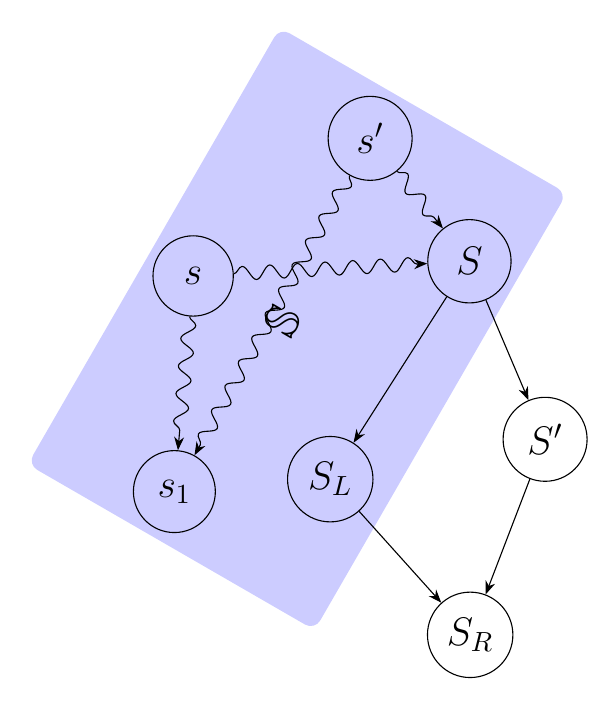
\begin{tikzpicture}
  \state{s}{}
  \state{s'}{above right = 1.0cm and 1.5cm of s}
  \state{s_1}{below left = 2.0cm and -0.5cm of s}
  \state{S}{below right = 0.8cm and 0.5cm of s'}
  \state{S'}{below right = 1.5cm and 0.2cm of S}
  \state{S_L}{below left = 2.0cm and 1.0cm of S}
  \state{S_R}{below right = 1.2cm and 1.0cm of S_L}

  \draw[path] (s) to (s_1);
  \draw[path] (s) to (S);

  \draw[path] (s') to (s_1);
  \draw[path] (s') to (S);

  \draw[edge] (S) to (S_L);
  \draw[edge] (S) to (S');

  \draw[edge] (S_L) to (S_R);
  \draw[edge] (S') to (S_R);

  \begin{pgfonlayer}{background}
	\node () [rectangle, rounded corners, inner sep = 5pt, rotate fit = 60, 
	  font = \LARGE, fill = blue!20,
	fit = (s) (s') (s_1) (S) (S_L)] {$\mathbb{S}$};
  \end{pgfonlayer}
\end{tikzpicture}
\end{document}
